\section{Results}

\subsection{The Galaxy Stellar Mass Function}

\begin{figure*}
	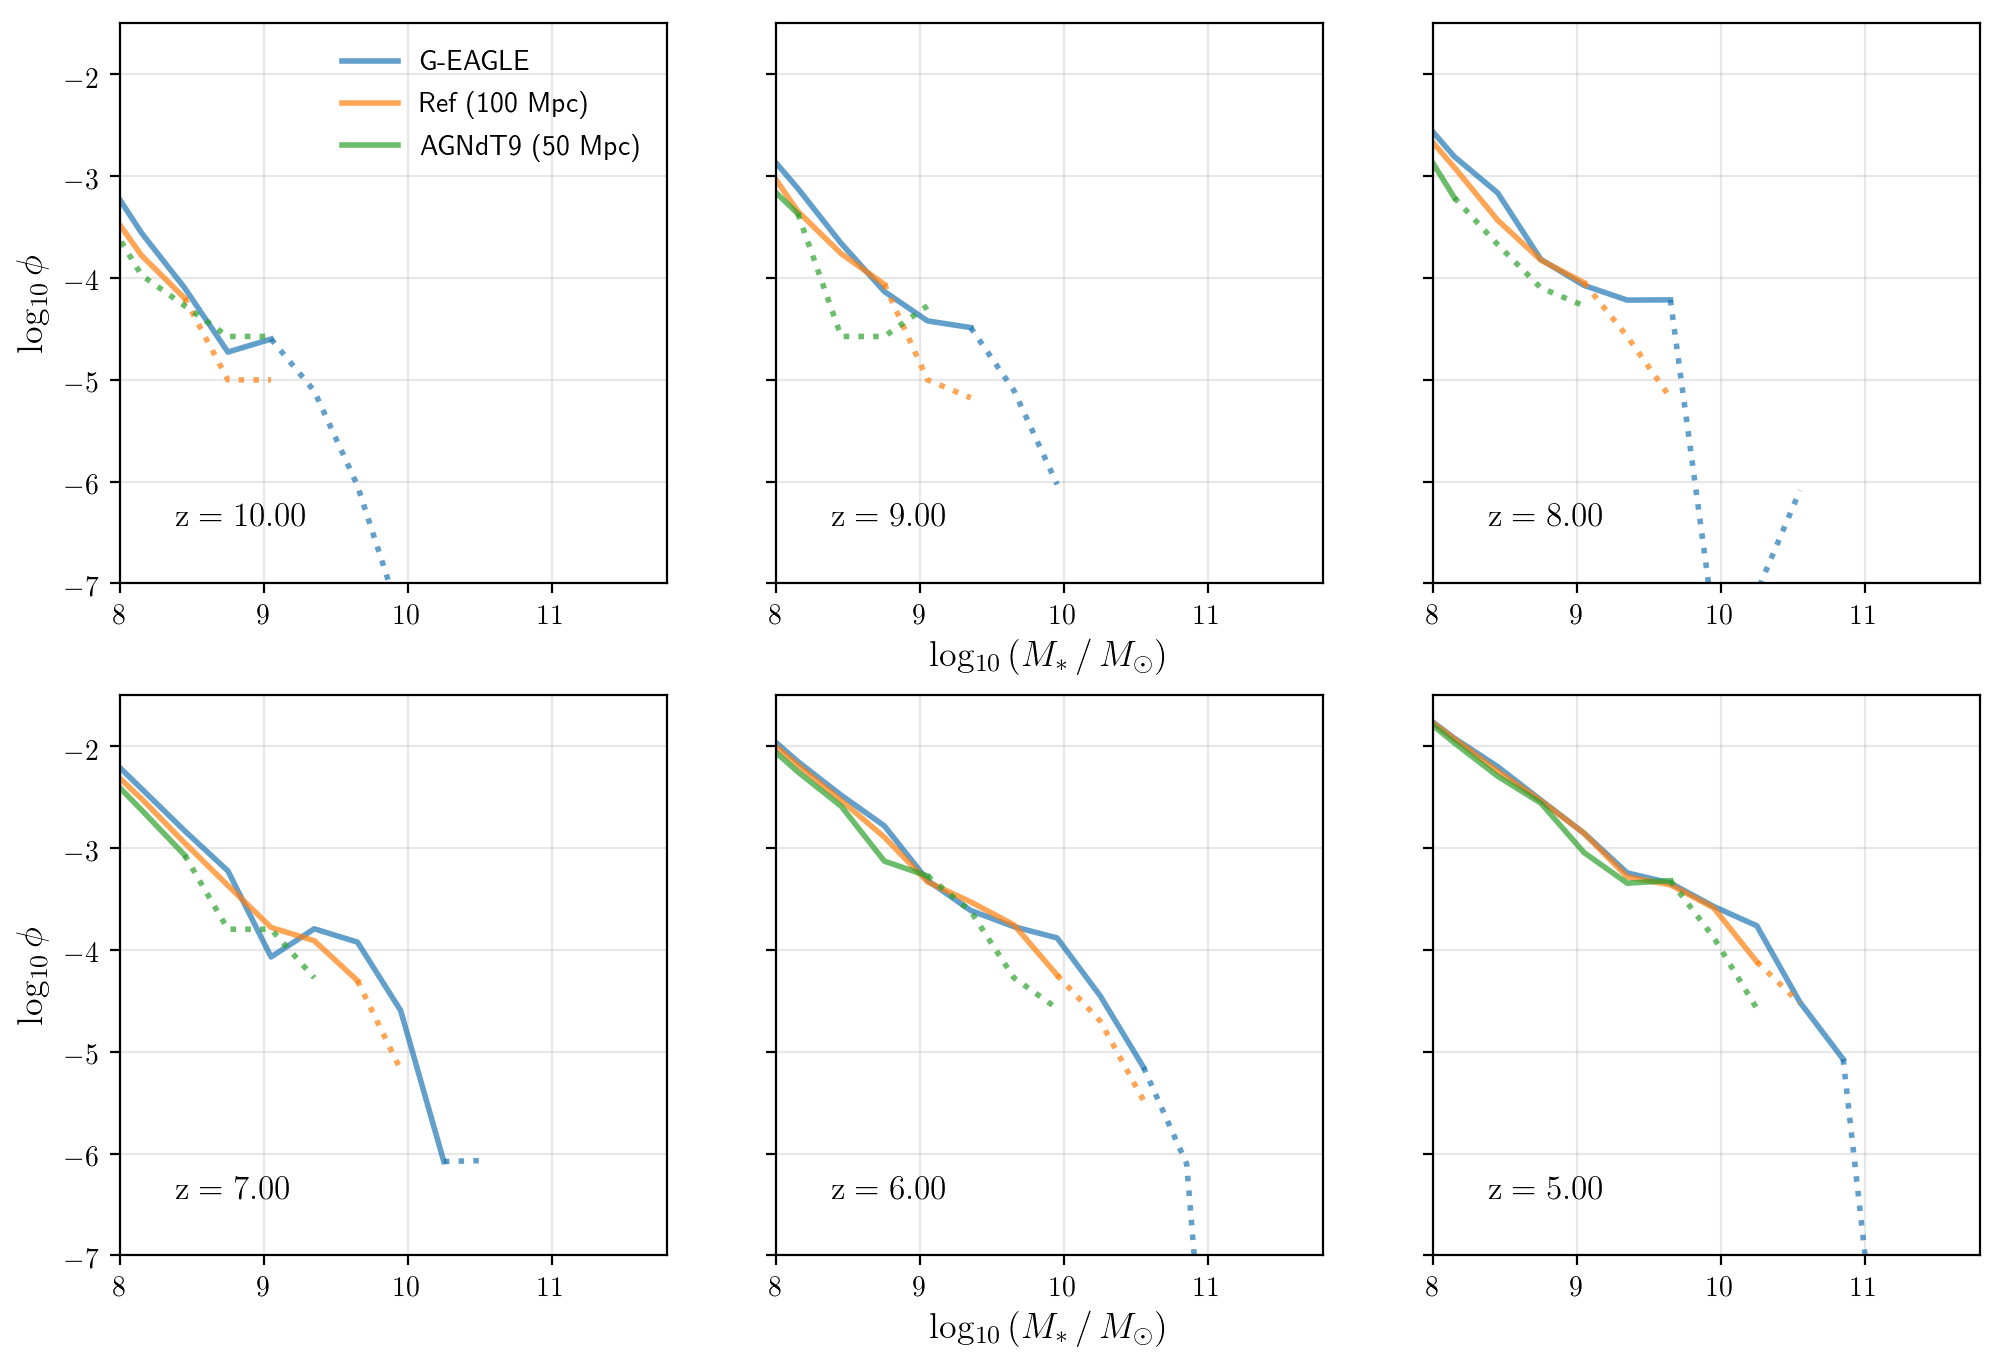
\includegraphics[width=\textwidth]{images/gsmf_multi.png}
    \caption{Galaxy stellar mass function.}
    \label{fig:gsmf_multi}
\end{figure*}

\fig{gsmf_multi} shows the Galaxy Stellar Mass Function for redshifts between $z = 5 \rightarrow 10$.
The composite \textsc{G-Eagle} GSMF is shown in blue, the Ref in orange, and the AGNdT9 50 Mpc volume in green.
It is clear that the composite mass function extends the dynamic range by approximately 0.8 dex at almost all redshifts.
At lower masses the composite mass function is in good agreement with that from the fiducial simulations, which demonstrates that our weighting scheme is correctly predicting the abundance of more common galaxies.

\begin{figure*}
	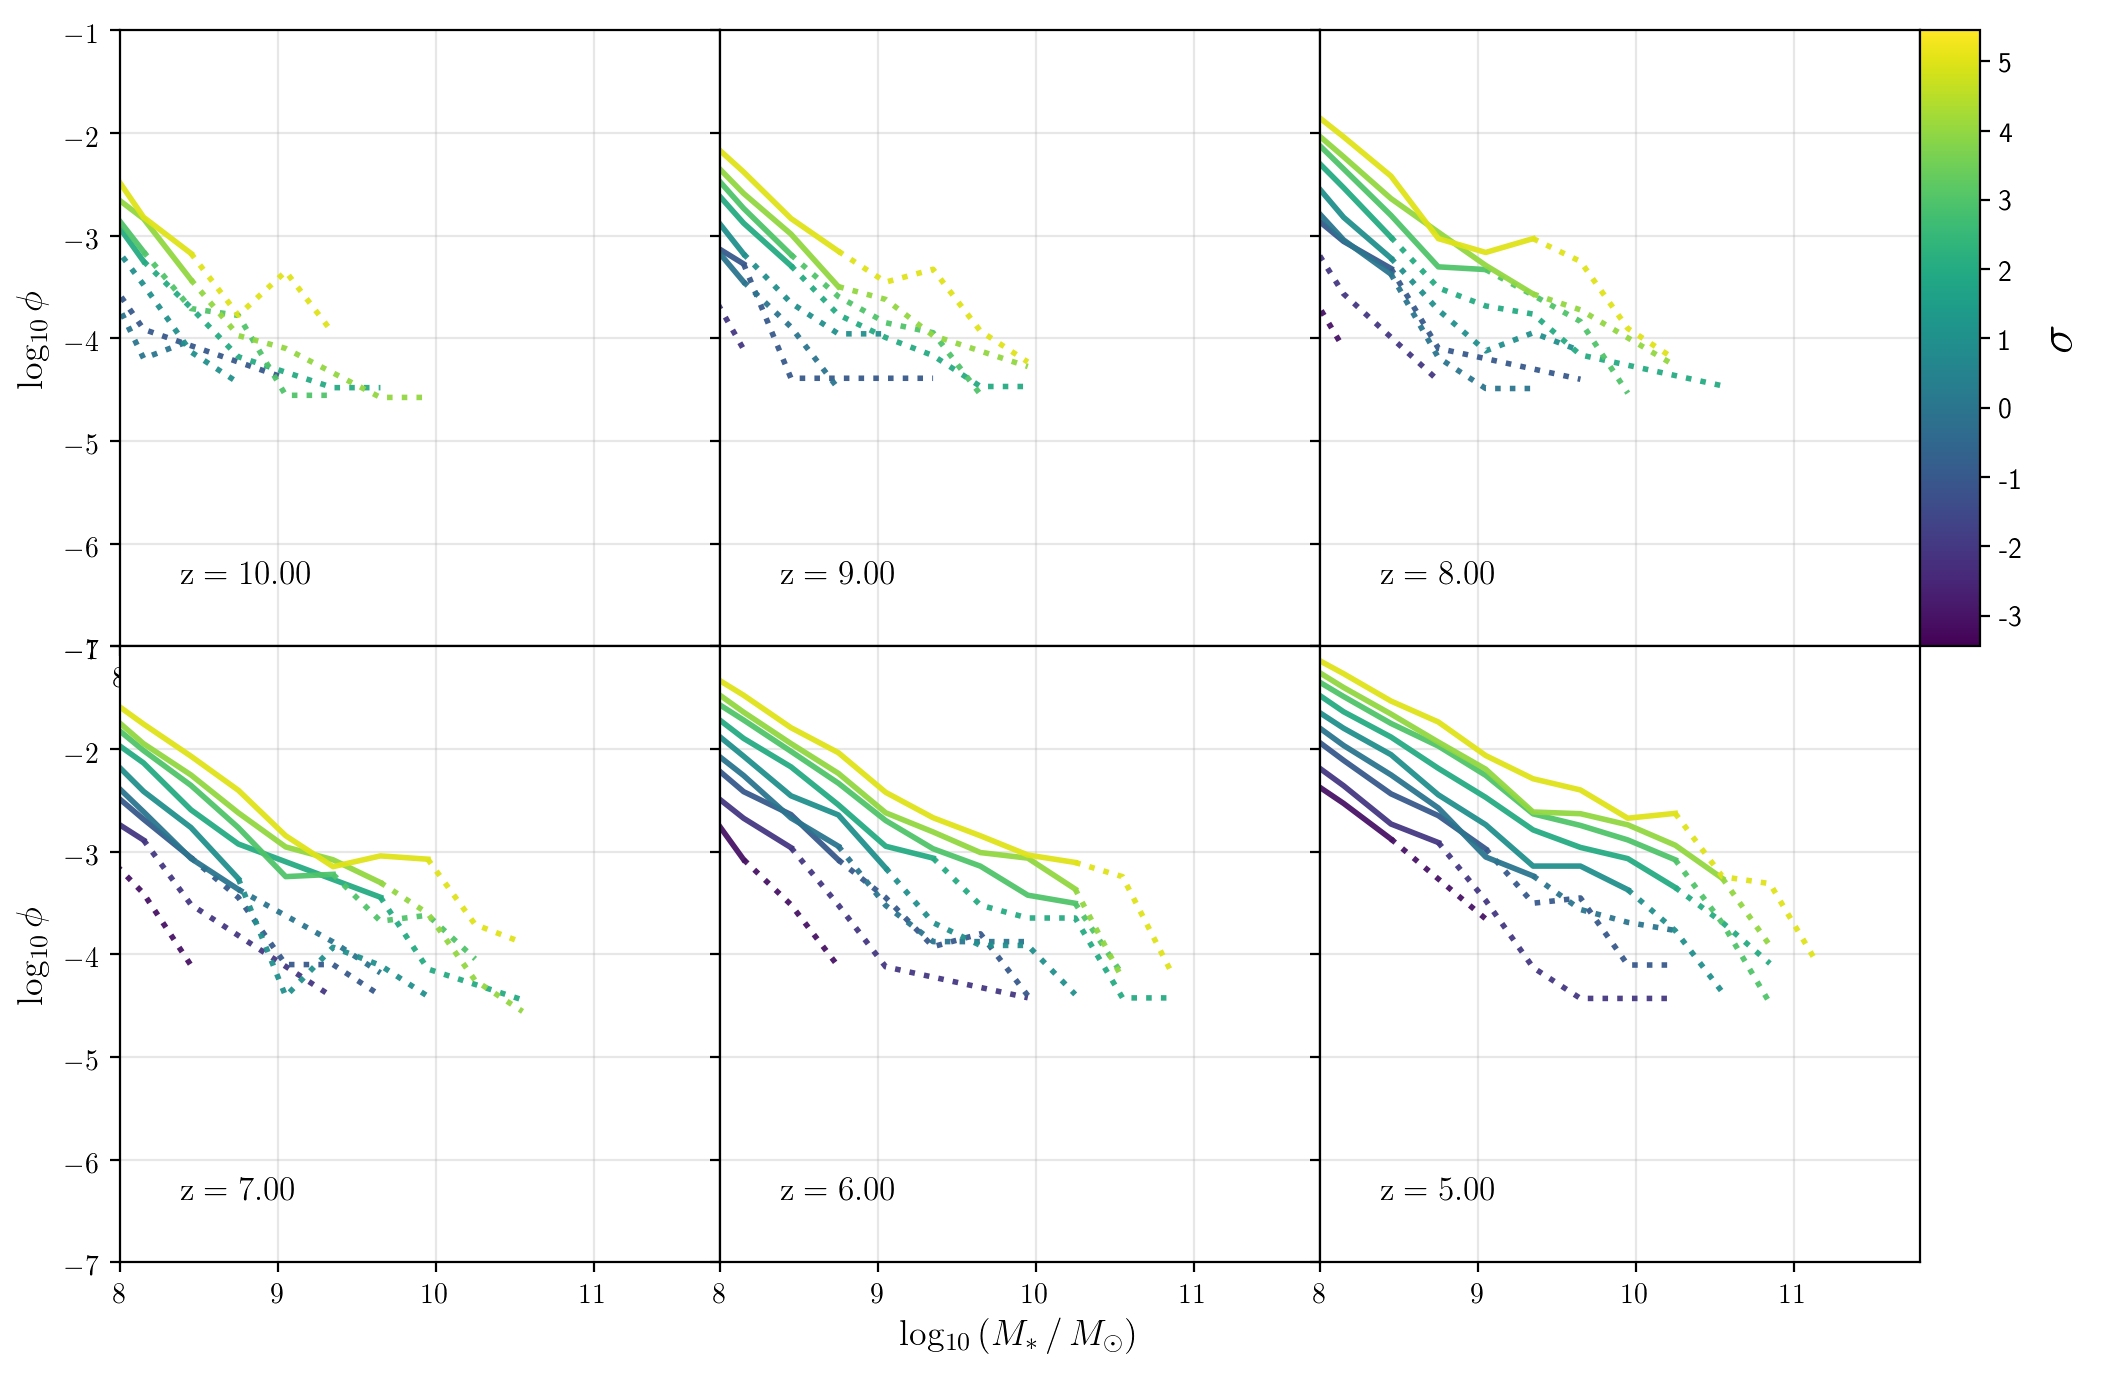
\includegraphics[width=\textwidth]{images/gsmf_multi_split.png}
    \caption{Galaxy stellar mass function, split by overdensity.}
    \label{fig:gsmf_multi_split}
\end{figure*}

\todo{GSMF for different environments}

\todo{update from thesis}
The Galaxy Stellar Mass Function (GSMF) describes the number of galaxies per unit volume per unit stellar mass interval $\mathrm{d}M$,
\begin{align}
    \mathrm{\phi(M)} = N \,/\, \mathrm{Mpc^{-3} \, dex^{-1}}\;\;,
\end{align}
and is commonly described using a Schechter function \citep{schechter_analytic_1976},
\begin{align}
    \phi(M) \, \mathrm{d}M = \phi_{*} \, \left( \frac{M}{M_{*}}\right)^{\alpha} \, \mathrm{exp}\left( \frac{-M}{M_{*}} \right) \frac{\mathrm{d}M}{M_{*}}\;\;,
\end{align}
which describes the high- and low-mass behaviour with an exponential and a power law dependence on stellar mass, respectively.
Recent studies have found that a double Schechter function can better fit the full distribution \citep[\textit{e.g.} the GAMA survey, ][]{baldry_galaxy_2008}.

\todo{Fit distribution function, show evolution with redshift and difference with overdensity}

\subsection{The Star Formation Rate Distribution Function}

\todo{composite SFRF}

\todo{SFRF for different environments}

\subsection{The Star-Forming Sequence}

\todo{update from thesis}
Observations suggest a close relationship between the star formation rate (SFR) and stellar mass of galaxies, at both high and low redshifts, which I will refer to as the star-forming sequence (SFS), though it also commonly referred to as the `main sequence' \citep{brinchmann_physical_2004,noeske_star_2007,speagle_highly_2014}.
The SFS is typically parametrised as a linear relation,
\begin{align}
  \mathrm{log_{10}(SFR)} = \alpha \; \mathrm{log_{10}(M_{*}\,/\, M_{\odot})} + \beta\;\;,
\end{align}
where the slope $\alpha$ remains relatively constant with increasing redshift, but the normalisation $\beta$ increases \citep{daddi_multiwavelength_2007, santini_star_2009, salmon_relation_2015}.
There have also been suggestions of a turnover in the SFS at high stellar masses \citep{lee_turnover_2015,tasca_evolving_2015}, though the turnover becomes less evident with increasing redshift.
This behaviour has been seen in both low redshift \citep{lee_turnover_2015} and high redshift \citep{tasca_evolving_2015, santini_star_2017} observations, but is absent from some models \citep[\textit{e.g.} Illustris, ][]{sparre_star_2015}.
The turnover may be evidence for a change in the dominant channel of stellar mass growth from smooth gas accretion to merger driven growth.
A high-mass SFS turnover is also necessary to explain the galaxy stellar mass function at lower stellar masses; a single power law slope would lead to too many massive galaxies being formed \citep{leja_reconciling_2015}.

\todo{composite SFS}

\todo{SFS for different environments}
